\documentclass[10pt,conference]{IEEEtran}
\IEEEoverridecommandlockouts

\usepackage{cite}
\usepackage{amsmath,amssymb}
\usepackage{graphicx}
\usepackage{booktabs}
\usepackage{multirow}
\usepackage{xcolor}
\usepackage{url}
\usepackage{array}
\usepackage[colorlinks=true, urlcolor=blue, linkcolor=blue, citecolor=blue]{hyperref}
\usepackage{tikz}
\usepackage{float}
\usepackage[section]{placeins}
\graphicspath{{images/}}

\usetikzlibrary{
    arrows.meta,
    positioning,
    fit,
    backgrounds
}

\newcommand{\wg}[1]{\textcolor{red}{#1}}

\begin{document}

\title{A Pose-Based AI Coach for Exercise Recognition and Quality Assessment
\thanks{This work is Funded by the Science and Technology Development Fund STDF (Egypt); Project id: 51399
- ``VERAS: Virtual Exercise Recognition and Assessment System''.}
\thanks{This work involved human subjects in its research. The author(s) confirm(s) that all human subject research procedures and protocols are exempt from review board approval. Participation was voluntary, verbal informed agreement was obtained from all volunteers, and all collected data were anonymized using numerical identifiers to preserve participant privacy.}}

\author{
\IEEEauthorblockN{Ahmed Aly}
\IEEEauthorblockA{\textit{Dept. of Computer Science and Engineering} \\
\textit{Egypt-Japan University of Science and Technology}\\
Alexandria, Egypt \\
ahmed.mohammad@ejust.edu.eg}
\and
\IEEEauthorblockN{Al Amir Eldomiatty}
\IEEEauthorblockA{\textit{Dept. of Computer Science and Engineering} \\
\textit{Egypt-Japan University of Science and Technology}\\
Alexandria, Egypt \\
alamir.eldomiatty@ejust.edu.eg}
\and
\IEEEauthorblockN{Zeyad Elsayed}
\IEEEauthorblockA{\textit{Dept. of Computer Science and Engineering} \\
\textit{Egypt-Japan University of Science and Technology}\\
Alexandria, Egypt \\
zeyad.elsayed@ejust.edu.eg}
\and
\IEEEauthorblockN{Walid Gomaa$^{1,2}$}
\IEEEauthorblockA{$^1$\textit{Egypt-Japan University of Science and Technology}\\
Alexandria, Egypt \\
$^2$Faculty of Engineering, Alexandria University,\\
Alexandria, Egypt
walid.gomaa@ejust.edu.eg}
}

\maketitle

\begin{abstract}
We present an AI Virtual Coach composed of: (i) Exercise Recognition, (ii) Exercise Assessment, and (ii) Coaching Agent.
The recognition module employs a systematic feature engineering approach, evolving from 19 base biomechanical features (joint angles and distances) to 37 view-specific specialized features fed into a Feedforward Neural Network designed to resolve persistent confusion clusters identified through multi-run experiments.
The assessment module performs aspect-level scoring for 15 resistance-training exercises using temporal pose sequences extracted from RGB video via MediaPipe, repetition segmentation, and a compact temporal CNN regressor.
We evaluate on our newly collected dataset of 51 volunteers (10 female, 41 male), captured simultaneously in front and side views using mobile phones.
Our 37-feature representation achieves 90.36\% macro F1 on side view and 86.94\% macro F1 on front view, with robust performance across all 15 exercise classes.
We use a subject-disjoint protocol and 30 randomized runs to ensure robust evaluation. This dataset represents a major contribution to the field of pose-based exercise assessment.
\end{abstract}

\begin{IEEEkeywords}
Virtual coach,  exercise recognition, action quality assessment, exercise assessment, Neural Network Applications, Industrial Applications, Interpretable and Explainable AI, rep segmentation, pose estimation, temporal CNN
\end{IEEEkeywords}

\section{Introduction}
\label{sec: Introduction}

\par 
Resistance training is widely practiced for improving strength, hypertrophy, and overall health, yet incorrect technique can reduce training effectiveness and increase injury risk. In-person coaching helps correct form, but it is expensive, time-constrained, and not always available. This motivates \emph{AI virtual coaching} systems that can provide scalable, low-cost feedback using commodity devices such as smartphones~\cite{vcoach, cameracoach, kaushik2024posture, sharshar2022mmdos}.

\par 
Recent progress in computer vision has enabled reliable \emph{exercise recognition} from video, answering the question of \emph{what} movement is being performed. However, virtual coaching also requires answering \emph{how well} an exercise is executed. This falls under \emph{action quality assessment} (AQA), where models estimate execution quality rather than only classifying the action. Most AQA research has focused on competitive sports or large-scale benchmarks, and commonly predicts a single overall score from a full clip. In contrast, gym training has distinct properties: videos often contain \emph{multiple repetitions} per set; execution quality may vary across repetitions; and coaches typically evaluate form across multiple \emph{aspects} (e.g., alignment, range of motion, stability, and control) rather than a single scalar rating. These differences make direct adoption of standard AQA pipelines suboptimal for practical fitness assessment~\cite{core, flex}.

\par
A further challenge is that deployable systems must operate in uncontrolled settings: consumer RGB video with varying camera placement, lighting, and occlusions. In small, real-world datasets, reliable evaluation is also difficult because performance can vary substantially across random initializations and subject splits. Finally, in many fitness datasets (including ours), supervision is available at the \emph{set/video level} (one label per volunteer per exercise set), not per repetition, which requires models to reconcile repetition-level inputs with subject-level targets~\cite{vcoach, cameracoach}.

\par 
    In this work, we study whether a lightweight, pose-based, multi-stage pipeline can provide practical assessment from consumer video under limited data. We propose an AI Virtual Coach composed of (i) an \emph{exercise recognition} model to identify the exercise performed, and (ii) an \emph{exercise assessment} model that predicts five aspect-level scores (0--10). The assessment module extracts temporal pose features, segments repetitions using exercise/view-specific biomechanical signals, encodes each repetition with a compact temporal CNN, and aggregates multiple repetition embeddings into a subject-level representation aligned with set-level labels; it then predicts \emph{five aspect-specific scores} on the 0--10 scale (one score per assessment criterion).
 We evaluate on a dataset of 51 volunteers performing 15 resistance-training exercises, recorded simultaneously from front and side viewpoints, and annotated by two certified coaches.

\par 
Our central research question is: \emph{Can explicit repetition modeling (segmentation and aggregation) combined with compact pose-based temporal modeling enable consistent, aspect-level exercise assessment from consumer RGB video, and how do front and side viewpoints compare under a subject-disjoint evaluation protocol?} Answering this question contributes evidence toward deployable virtual coaching in realistic gym settings, and provides a reproducible evaluation protocol for small fitness-assessment datasets.

Our contributions are as follows:
\begin{itemize}
  \item A 37-dimensional view-specific feature representation combining biomechanical joint angles with specialized discrimination features targeting exercise-specific confusion patterns (curl grip, hinge dynamics, arm extension depth, elevation detection).
  \item A practical modular virtual-coach pipeline integrating exercise recognition, per-repetition assessment, and LLM-based coaching feedback.
  \item A subject-disjoint multi-run evaluation protocol (30 runs) achieving 90.36\% macro F1 (side) and 86.94\% macro F1 (front) for 15-class exercise recognition.
\end{itemize}

\par
\textbf{Data and Code Availability.} The code for this work is publicly available at \url{https://github.com/AhmedAly0/AI-Virtual-Coach}. The dataset is available upon reasonable request.

The remainder of this paper is organized as follows. Section~\ref{sec: Related Work} reviews related work in action quality assessment and pose-based analysis. Section~\ref{sec: Methods} describes our dataset and methodology, including the proposed pose-based feature engineering and assessment pipeline. Section~\ref{sec: Experimental Setup} details the experimental setup and evaluation protocols. Finally, Section~\ref{sec: Results and Discussion} presents the results and discussion, and Section~\ref{sec: Conclusion} concludes the paper.


\section{Related Work}
\label{sec: Related Work}

\subsection{Action Quality Assessment}

Action Quality Assessment (AQA) aims to predict execution quality rather than just recognizing action categories~\cite{core, flex}. Traditional AQA maps videos to scalar scores, but recent approaches improve this by modeling relative quality or leveraging human-AI collaboration. For instance, CoRe~\cite{core} uses contrastive regression to predict relative feature differences, while SkillNet~\cite{roy2026skillnet} incorporates expert feedback for fine-grained skill assessment. These methods typically rely on global clip context, whereas fitness coaching often requires repetition-level granularity.

\subsection{Fitness AQA Datasets and Structured Supervision}

Recent work emphasizes fitness-specific datasets with richer supervision. FLEX~\cite{flex} provides a large-scale multimodal (RGB, pose, sEMG) dataset with auditable expert annotations. Similarly, systems like VCOACH and Camera Coach~\cite{vcoach, cameracoach, sharshar2022mmdos} utilized the MM-DOS dataset to demonstrate the value of fusing RGB, thermal, and depth data for robust assessment. More recently, ALEX-GYM-1~\cite{hassan2025alexgym} introduced hybrid vision-landmark models for automated evaluation. Our work complements these multimodal benchmarks by focusing on a lightweight, deployable pipeline using only consumer-grade RGB cameras (front/side) and subject-disjoint evaluation on real-world data, prioritizing accessibility over specialized sensor setups.

\subsection{Pose-Based Motion Modeling}

Pose extraction via tools like MediaPipe~\cite{mediapipe} enables low-cost kinematic analysis. Recent impactful applications include AI-based posture correction systems~\cite{kaushik2024posture} and attention-based gait recognition models like Gait-ViT~\cite{gaitvit}, which demonstrate the power of temporal dynamics in motion analysis. In our setting, we adopt a compact temporal CNN over resampled joint-angle sequences to balance modeling capacity with dataset scale and deployment constraints, incorporating explicit repetition parsing to align representations with resistance training cycles.





\section{Methods}
\label{sec: Methods}

\par 
This section describes our data collection process, pose feature extraction pipeline, and the proposed models for exercise recognition, exercise assessment and the coaching agent.

\subsection{Data Collection}

\subsubsection{Participants}

The dataset was collected from 51 recreationally active volunteers, including 41 males (80.4\%) and 10 females (19.6\%). The observed gender imbalance reflects practical constraints related to video-based data collection in public gym environments in Egypt, where a proportion of female gym members preferred not to be recorded. Participation was entirely voluntary, and only individuals who explicitly agreed to video recording were included.
All participants reported no current musculoskeletal injuries at the time of recording.Summary statistics of participant demographics and anthropometric measurements are provided in Table~\ref{tab:participants}.
\begin{table}[H]
\caption{Participant Demographics and Anthropometric Statistics}
\label{tab:participants}
\centering
\begin{tabular}{lccc}
\hline
\textbf{Attribute} & \textbf{Min} & \textbf{Max} & \textbf{Mean $\pm$ SD} \\
\hline
Age (years) & 15 & 29 & 21.3 $\pm$ 3.1 \\
Height (cm) & 158 & 190 & 174.2 $\pm$ 7.6 \\
Weight (kg) & 52 & 110 & 77.5 $\pm$ 13.9 \\
BMI (kg/m$^2$) & 18 & 37 & 24.7 $\pm$ 4.1 \\
\hline
\end{tabular}
\end{table}

\subsubsection{Exercise set}

\par 
The dataset includes recordings of 15 resistance training exercises covering both upper- and lower-body movements: 
\textit{Dumbbell Shoulder Press, Hammer Curls, Standing Dumbbell Front Raises, Lateral Raises, Bulgarian Split Squat, EZ-Bar Curls, Incline Dumbbell Bench Press, Overhead Triceps Extension, Shrugs, Weighted Squats, Seated Biceps Curls, Triceps Kickbacks, Rows, Deadlift, Calf Raises.}

\par 
Overall, the dataset contains a larger variety of upper-body exercise types than lower-body exercise types. However, the number of volunteers contributing to each exercise was approximately comparable across upper- and lower-body movements, reflecting natural participation during the recording sessions.


\subsubsection{Recording setup and protocol}

\par 
All recordings were conducted indoors at multiple local gym facilities in Egypt. Videos were captured using a smartphone camera at a resolution of 1080~$\times$~1920 pixels and a frame rate of 30 frames per second, in landscape orientation. Lighting conditions varied across sessions, resulting in mixed indoor illumination.

\par 
Camera height and distance were not strictly fixed and varied depending on the exercise, though recordings generally captured either the full body or were positioned at approximately waist level. Each video corresponds to a single exercise set lasting approximately 30 to 60 seconds and containing 8 to 12 repetitions, recorded as a continuous sequence.

\par 
Participants performed exercises using self-selected weights to emulate realistic training conditions. Exercise execution was performed naturally, allowing for intra- and inter-subject variability in movement quality, which is essential for form assessment modeling.


\subsubsection{Viewpoint acquisition}

\par 
To capture complementary kinematic information, each exercise was recorded from two viewpoints: \textbf{Front view and Side view}


A total of 154 videos per viewpoint were recorded, resulting in 308 videos overall. Each video was segmented into repetition-level clips, where each clip corresponds to a single exercise repetition. Viewpoints were manually labeled during preprocessing.


\subsubsection{Expert annotation}

\par 
Each recorded exercise set was annotated by two certified fitness coaches using  reliability-weighted label $y=0.25y_{C1}+0.75y_{C2}$ based on a joint review of the corresponding front-view and side-view videos. Annotations were performed at the video (set) level, rather than at the individual repetition level.

\par 
For each exercise, coaches evaluated five predefined biomechanical aspects specific to that movement, such as joint alignment, range of motion, stability, and movement control. These criteria were defined in advance for each exercise to ensure consistency across annotations.
The resulting annotation scores represent an overall quality assessment of the exercise set and were used as supervisory signals for training and evaluating the proposed exercise assessment model. Repetition-level clips extracted from each video inherit the corresponding set-level annotation.


\subsubsection{Dataset limitations}

\par 
The dataset exhibits a gender imbalance, with a higher proportion of male participants, as well as a limited number of lower-body exercise samples. These limitations are primarily due to cultural and logistical constraints during data collection. Nevertheless, the dataset captures substantial inter-subject variability and realistic execution patterns, making it suitable for evaluating virtual coaching and exercise assessment systems.


\subsection{System Overview}

\par 
Fig.~\ref{fig:pipeline} illustrates the end-to-end pipeline of our AI Virtual Coach. The system processes a single-view RGB video (either front or side) and produces structured textual feedback through four sequential stages.

\par 
\textbf{Stage 1: Pose Estimation and Feature Extraction.}
Given an input video, we extract 3D pose landmarks for each frame using MediaPipe Pose Landmarker. The raw landmarks are normalized for scale and translation invariance (Section~\ref{sec:pose_gen}), and nine biomechanical joint angles are computed per frame. The resulting temporal sequence is resampled to a fixed length of $T=50$ timesteps, yielding a feature tensor of shape $(50, 9)$ per repetition.

\par 
\textbf{Stage 2: Exercise Recognition.}
The temporal pose features are passed to a Feedforward Neural Network classifier that identifies which of the 15 supported exercises is being performed. The predicted exercise class determines which exercise-specific assessment model to invoke, enabling specialized evaluation tailored to each movement's biomechanics.

\par 
\textbf{Stage 3: Per-Repetition Assessment.}
Based on the recognized exercise, the corresponding assessment model (one of 15 trained separately per exercise and view) evaluates each detected repetition. Rather than outputting a single aggregated score, the model produces \emph{per-repetition} scores for five exercise-specific aspects (e.g., joint alignment, range of motion, tempo, stability). This fine-grained output enables downstream analysis of form consistency and fatigue patterns across the set.

\par 
\textbf{Stage 4: Coaching Agent.}
The per-rep assessment scores, along with exercise-specific evaluation criteria, are passed to a stateful coaching agent implemented using LangGraph. The agent performs rule-based trend analysis to detect fatigue (by comparing early vs.\ late reps), computes a consistency score (inverse of score variance), and identifies the strongest and weakest aspects. These analytical results, together with the detailed per-rep breakdown, are then passed to a large language model (Google Gemini 2.5 Flash) that generates personalized, actionable coaching feedback in natural language. The final output includes aggregated scores, trend indicators, fatigue warnings, and a conversational feedback summary suitable for display in a mobile application.

\begin{figure*}[t]
\centering
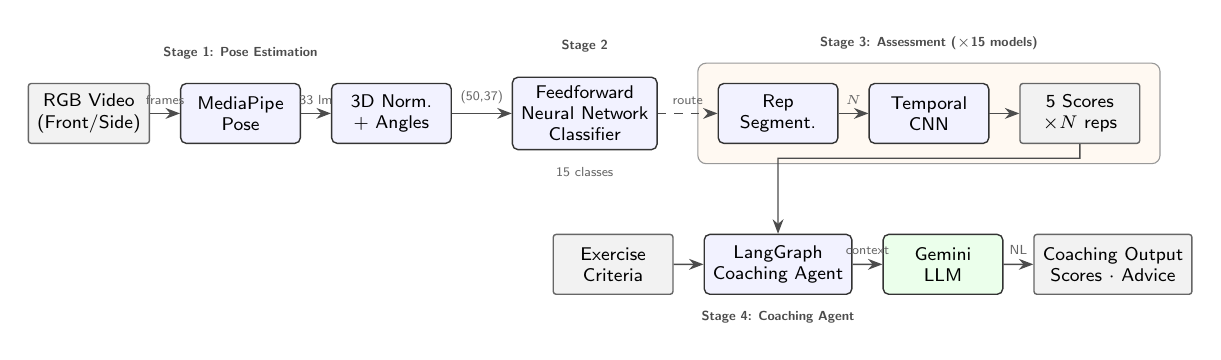
\begin{tikzpicture}[scale=0.95, transform shape,
    font=\sffamily\scriptsize,
    node distance=4mm,
    box/.style={
        rectangle,
        rounded corners=2pt,
        draw=black!80,
        fill=blue!5,
        line width=0.5pt,
        align=center,
        minimum height=8mm,
        minimum width=16mm
    },
    data/.style={
        rectangle,
        rounded corners=1pt,
        draw=black!60,
        fill=gray!10,
        line width=0.5pt,
        align=center,
        minimum height=8mm,
        minimum width=16mm
    },
    stage/.style={
        font=\sffamily\tiny\bfseries,
        text=black!70
    },
    annot/.style={
        font=\sffamily\tiny,
        text=black!60
    },
    arrow/.style={->, >=Stealth, line width=0.5pt, black!70},
    dashedarrow/.style={->, >=Stealth, dashed, line width=0.5pt, black!70}
]

% ===== ROW 1: Stages 1-3 =====
\node[data] (rgb) {RGB Video\\(Front/Side)};
\node[box, right=of rgb] (mp) {MediaPipe\\Pose};
\node[box, right=of mp] (norm) {3D Norm.\\+ Angles};
\node[box, right=8mm of norm] (mlp) {Feedforward\\Neural Network\\Classifier};
\node[box, right=8mm of mlp] (rep) {Rep\\Segment.};
\node[box, right=of rep] (cnn) {Temporal\\CNN};
\node[data, right=of cnn] (score) {5 Scores\\$\times N$ reps};

\draw[arrow] (rgb) -- node[annot, above]{frames} (mp);
\draw[arrow] (mp) -- node[annot, above]{33 lm} (norm);
\draw[arrow] (norm) -- node[annot, above]{(50,37)} (mlp);
\draw[dashedarrow] (mlp) -- node[annot, above]{route} (rep);
\draw[arrow] (rep) -- node[annot, above]{$N$} (cnn);
\draw[arrow] (cnn) -- (score);

% Stage labels (row 1)
\node[stage, above=2mm of mp] {Stage 1: Pose Estimation};
\node[stage, above=2mm of mlp] {Stage 2};
\node[annot, below=1mm of mlp] {15 classes};

% Stage 3 bounding box
\begin{scope}[on background layer]
\node[
    draw=black!40,
    rounded corners=3pt,
    line width=0.4pt,
    fill=orange!5,
    fit=(rep)(cnn)(score),
    inner sep=2.5mm,
    label={[stage, above=0.5mm]north:Stage 3: Assessment ($\times$15 models)}
] {};
\end{scope}

% ===== ROW 2: Stage 4 =====
\node[box, below=12mm of rep] (agent) {LangGraph\\Coaching Agent};
\node[data, left=of agent] (crit) {Exercise\\Criteria};
\node[box, right=of agent, fill=green!8] (llm) {Gemini\\LLM};
\node[data, right=of llm, minimum width=20mm] (out) {Coaching Output\\Scores $\cdot$ Advice};

\draw[arrow] (score) -- ++(0,-6mm) -| (agent);
\draw[arrow] (crit) -- (agent);
\draw[arrow] (agent) -- node[annot, above]{context} (llm);
\draw[arrow] (llm) -- node[annot, above]{NL} (out);

\node[stage, below=1mm of agent] {Stage 4: Coaching Agent};

\end{tikzpicture}
\caption{End-to-end pipeline. Stage~1 extracts pose landmarks and computes 37 biomechanical features. Stage~2 classifies the exercise (15 classes). Stage~3 segments repetitions and applies exercise-specific temporal CNN models for per-rep aspect scores. Stage~4 uses LangGraph with Gemini LLM for personalized feedback.}
\label{fig:pipeline}
\end{figure*}

\subsection{Pose Data Generation}
\label{sec:pose_gen}

\subsubsection{Pose landmark extraction}

\par 
For each video frame, 3D human pose landmarks were extracted using the MediaPipe Pose Landmarker Lite model~\cite{mediapipe}. The model produces 33 body landmarks per frame, each with $(x, y, z)$ coordinates, where $x$ and $y$ represent normalized image-plane coordinates and $z$ represents depth from the camera plane. Detection and tracking confidence thresholds were set to 0.3. Frames were converted from BGR to RGB color space for MediaPipe compatibility, and a fresh \texttt{PoseLandmarker} instance was created per video to ensure proper timestamp handling in VIDEO mode.

\subsubsection{3D landmark normalization}
To achieve scale and translation invariance with respect to camera distance and subject body size, all landmarks were normalized in 3D space using a torso-length-based transformation. First, the pelvis center $\mathbf{p}$ was computed as the midpoint of the left hip (landmark 23) and right hip (landmark 24):
\begin{equation}
\mathbf{p} = \frac{1}{2}(\mathbf{h}_{23} + \mathbf{h}_{24}),
\end{equation}
where $\mathbf{h}_{i} = (x_i, y_i, z_i)$. Similarly, the mid-shoulder point $\mathbf{s}$ was computed as the midpoint of the left shoulder (landmark 11) and right shoulder (landmark 12):
\begin{equation}
\mathbf{s} = \frac{1}{2}(\mathbf{h}_{11} + \mathbf{h}_{12}).
\end{equation}
The torso length $L$ in 3D space was then calculated as:
\begin{equation}
L = \|\mathbf{s} - \mathbf{p}\| = \sqrt{(s_x - p_x)^2 + (s_y - p_y)^2 + (s_z - p_z)^2}.
\end{equation}
Finally, each landmark $\mathbf{h}_i$ was normalized as:
\begin{equation}
\mathbf{h}_i^{\text{norm}} = \frac{\mathbf{h}_i - \mathbf{p}}{L}.
\end{equation}
Frames with invalid torso length ($L < 10^{-6}$) were discarded to ensure numerical stability.

\subsection{Feature Engineering}
\label{sec:feature_eng}

\par 
A central contribution of our work is a systematic feature engineering approach that evolves from basic joint angles to specialized discrimination features targeting specific confusion patterns.

Our methodology follows a data-driven iterative process: (i) establish baseline performance with fundamental biomechanical features, (ii) analyze confusion matrices to identify persistent misclassification clusters, and (iii) design targeted features grounded in exercise biomechanics to resolve each cluster.

\subsubsection{Base Feature Set}

\par 
The base feature set comprises 13 joint angles and 6 distance-based features, computed from normalized 3D landmarks.

\par 
\textbf{Joint Angles (13 features).} For each angle defined by a triplet of landmarks $(a, b, c)$ where $b$ is the joint vertex, the angle $\theta$ was calculated using the 3D dot product formula:
\begin{equation}
\theta = \arccos\left(\frac{\mathbf{v}_1 \cdot \mathbf{v}_2}{\|\mathbf{v}_1\| \|\mathbf{v}_2\|}\right),
\end{equation}
where $\mathbf{v}_1 = \mathbf{h}_a - \mathbf{h}_b$ and $\mathbf{v}_2 = \mathbf{h}_c - \mathbf{h}_b$. The 13 angles comprise: bilateral elbow flexion (shoulder$\rightarrow$elbow$\rightarrow$wrist), bilateral shoulder abduction (elbow$\rightarrow$shoulder$\rightarrow$hip), bilateral hip flexion (shoulder$\rightarrow$hip$\rightarrow$knee), bilateral knee flexion (hip$\rightarrow$knee$\rightarrow$ankle), bilateral ankle dorsiflexion (knee$\rightarrow$ankle$\rightarrow$heel), bilateral wrist angles (elbow$\rightarrow$wrist$\rightarrow$pinky), and torso lean from vertical. 

\par
\textbf{Distance Features (6 features).} To capture spatial relationships not encoded by angles, we compute: (i) bilateral ear-to-shoulder vertical distance for detecting shoulder elevation (shrugs), (ii) bilateral wrist-to-shoulder Euclidean distance for arm extension, and (iii) bilateral elbow-to-hip distance for arm tuck position. These features address exercises where joint angles remain relatively constant but body segment positions change significantly.

\subsubsection{View-Specific Specialized Features}

\par
A key insight from our experiments is that different camera angles capture different aspects of exercise movements. While the same 33 landmarks are extracted from both views, the discriminative information differs substantially. The front view captures arm width, bilateral symmetry, and depth-axis movements, while the side view better captures elbow flexion, torso lean, and sagittal-plane trajectories. This motivated the development of \emph{view-specific} specialized features.

\par 
\subsubsection{Confusion-Driven Feature Design (Front View)}
Analysis of aggregated confusion matrices from 30-run experiments on the front view revealed four persistent confusion clusters requiring targeted intervention:

\textbf{Cluster 1: Curl Variants (30--35\% cross-prediction).} Hammer Curls, EZ-Bar Curls, and Seated Biceps Curls were frequently confused because their elbow flexion patterns are nearly identical. We designed 8 features targeting grip and arm position differences: (i) \emph{forearm supination} estimated from the hand plane normal ($\vec{n} = (\text{wrist}\rightarrow\text{index}) \times (\text{wrist}\rightarrow\text{thumb})$), distinguishing neutral grip (Hammer: $\sim$0°), angled grip (EZ-Bar: $\sim$30--45°), and full supination (Seated: $\sim$90°); (ii) \emph{upper arm vertical angle} capturing the inclined bench position in Seated Curls; (iii) \emph{inter-wrist distance} exploiting the fixed bar width in EZ-Bar Curls; and (iv) \emph{elbow-body distance} distinguishing tucked (EZ-Bar) versus flared (Hammer) elbow positions.

\par 
\textbf{Cluster 2: Hinge Movements ($\sim$25\% cross-prediction).} Deadlift and Bent-Over Rows share similar bent-over postures but differ in movement dynamics. We designed 4 features: (i) \emph{shoulder-width ratio} (shoulder width/hip width), which increases during row movements due to scapular retraction; (ii) \emph{wrist-hip vertical distance}, capturing the bar rising pattern in deadlifts versus the arm-pulling pattern in rows; and (iii) \emph{hip-depth ratio} (hip height/knee height), which changes throughout deadlifts but remains constant in rows.

\par 
\textbf{Cluster 3: Arm Extensions ($\sim$22\% cross-prediction).} Triceps Kickbacks and Rows both involve bent-over arm movements. We exploit the Z-axis (depth) difference: in kickbacks, the wrist moves \emph{posterior} to the hip ($z_{\text{wrist}} > z_{\text{hip}}$), while in rows the wrist remains beside the hip.

\par 
\textbf{Cluster 4: Minimal Motion ($\sim$16\% cross-prediction).} Shrugs and Calf Raises both exhibit minimal joint angle changes, making them indistinguishable by angle-based features alone. We designed 4 elevation features: (i) \emph{heel elevation} (heel height relative to foot index) captures plantar flexion in calf raises, and (ii) \emph{shoulder-center Y-position} captures shoulder elevation in shrugs. This demonstrates that some exercises require \emph{positional} rather than \emph{angular} features.

\subsubsection{Side-View Specialized Features}

\par 
For the side view, baseline experiments achieved 89.26\% accuracy but revealed critical underperformance in Shrugs (F1 = 0.59) and Overhead Triceps Extension (F1 = 0.65). We designed 18 side-view-specific features organized into 5 groups:

\par 
\textbf{Group 1: Vertical Displacement (4 features)} targets Shrugs versus Calf Raises using shoulder elevation, heel ground clearance, shoulder-hip Y ratio, and ear-shoulder compression.

\par 
\textbf{Group 2: Overhead Arm Position (4 features)} targets Overhead Triceps Extension using elbow-above-shoulder distance, wrist-above-elbow distance, and upper arm/forearm angles from vertical.

\par
\textbf{Group 3: Sagittal Arm Trajectory (4 features)} captures front-to-back arm movement patterns for discriminating curls, presses, and raises.

\par 
\textbf{Group 4: Hip Hinge Profile (4 features)} distinguishes Deadlift, Rows, and Kickbacks using torso angle from vertical, hip-ankle depth alignment, and shoulder-hip forward displacement.

\par 
\textbf{Group 5: Postural Stability (2 features)} provides general context through stance width and center-of-mass height.

\par 
A key design principle for side-view features is preferring Y-axis (vertical) measurements over Z-axis (depth), since the side camera angle captures vertical motion reliably but depth less accurately.

\subsubsection{Temporal feature representation}

\par 
For each exercise repetition, the nine joint angle timeseries were resampled to a fixed temporal length of $T_{\text{fixed}} = 50$ frames using linear interpolation to enable batch processing and model training. Let $\theta_j^{(t)}$ denote the $j$-th angle at original time index $t \in [0, T_{\text{orig}}-1]$. We defined a normalized time axis $\tau \in [0, 1]$ and applied linear interpolation to obtain angle values at target time indices $\tau' \in [0, 1]$ uniformly spaced with $T_{\text{fixed}}$ points. This resampling process produced temporal feature tensors of shape $(N_{\text{reps}}, 50, 37)$, where $N_{\text{reps}}$ is the total number of repetitions across all volunteers and exercises.

\par 
Edge cases were handled as follows: sequences with $T_{\text{orig}} = 0$ were filled with zeros, single-frame sequences ($T_{\text{orig}} = 1$) were replicated across all 50 timesteps, and sequences with $T_{\text{orig}} > 1$ underwent standard linear interpolation.

\subsubsection{Tempo preservation}

\par 
Since resampling to a fixed length inherently discards information about exercise execution speed, we explicitly preserved tempo as separate feature arrays. For each repetition, we computed: (i) \textbf{tempo\_duration\_sec}, the FPS-normalized duration in seconds calculated as $D = T_{\text{orig}} / \text{FPS}$, where $\text{FPS}$ is the video frame rate; (ii) \textbf{tempo\_frame\_count}, the total number of frames in the original video; and (iii) \textbf{tempo\_fps}, the original video FPS. These tempo features allow the model to distinguish between fast and slow executions of the same exercise, which is critical for movement quality assessment.

\subsection{Exercise Recognition}

\par 

The exercise recognition module classifies 15 resistance training exercises from temporal pose sequences using a feedforward neural network. This module processes the specialized features described in Section~\ref{sec:feature_eng}, performing subject-disjoint classification to ensure generalization to unseen individuals.

\subsubsection{Model architecture}

\par 
The temporal pose sequences of shape $(N_{\text{reps}}, 50, F)$ were flattened into $50F$-dimensional feature vectors, where $F=19$ for the base feature set or $F=37$ for the extended feature set with view-specific specialized features. Each vector represents the concatenated 
timeseries of biomechanical features over 50 timesteps. A feedforward neural network with three hidden layers was employed, with layer sizes of 512, 256, and 128 neurons respectively for the 37-feature configuration. Each hidden layer was followed by ReLU activation and dropout regularization with a dropout rate of 0.35 to prevent overfitting. The output layer consisted of 15 neurons with softmax activation for multi-class classification.

\subsubsection{Training protocol}

\par 
The model was trained using the Adam optimizer with a learning rate of $8 \times 10^{-5}$ and a batch size of 16. We utilize a stratified 3-way subject-independent split, ensuring that training, validation, and test sets contain data from strictly different participants (\textbf{subject-disjoint}) to test true generalization to unseen subjects. Training was conducted for a maximum of 200 epochs with early stopping monitoring validation loss, using a patience of 15 epochs and restoring the best weights upon convergence. Learning rate reduction on plateau was enabled with a factor of 0.5 and a patience of 10 epochs. The loss function was sparse categorical cross-entropy, and both accuracy and macro-averaged F1 score were monitored during training.

\subsection{Assessment Module}

\par 
Our assessment framework converts raw exercise videos into \emph{subject-level} performance scores through four stages: pose-based feature construction, repetition segmentation, repetition-to-subject aggregation, and multi-aspect regression. Pose preprocessing and temporal feature representation are described in Section~III-B.

\subsubsection{Pose extraction and feature representation}

\par 
From each repetition, we use the temporal joint-angle features described in Section~III-B, yielding a tensor of shape $(N_{\text{reps}}, 50, 9)$ (nine joint-angle signals over $T=50$ time steps). Since resampling to a fixed length removes absolute speed information, we preserve repetition tempo as separate metadata (e.g., repetition duration in seconds and original frame count), which can be fused with learned embeddings when needed.

\subsubsection{Repetition segmentation via exercise/view-specific signals}

\par 
We segment repetitions from the pose stream using an exercise/view-specific 1D ``rep signal'' designed to capture the primary biomechanical cycle of the movement (e.g., arm elevation for raises/pressing, elbow flexion for curls, and hip/knee depth for squats and split squats). The rep signal is smoothed and repetitions are detected using a robust threshold-based cycle logic (up--down--up or down--up--down) with:
(i) adaptive thresholds computed from within-video statistics to handle subject variability,
(ii) hysteresis to prevent rapid state flipping near thresholds, and
(iii) minimum-duration and minimum-separation constraints to reduce double counting due to noise.
This produces a variable number of repetitions $N_{\text{reps}}$ per video.

\subsubsection{Subject-level aggregation of multiple repetitions}

\par 
Because labels are provided at the set/video level (not per repetition), we aggregate multiple repetitions from the same volunteer into a single subject-level sample. Each repetition window (a $50 \times 9$ joint-angle sequence) is first encoded into an embedding $e_r \in \mathbb{R}^d$ using the temporal CNN encoder (1D convolutions over time followed by pooling to obtain a fixed-dimensional representation). We then perform masked attention pooling to handle the variable $N_{\text{reps}}$:
\begin{equation}
\alpha_r = \frac{m_r \exp(a(e_r))}{\sum_k m_k \exp(a(e_k))}, \qquad
e_{\text{subj}} = \sum_r \alpha_r e_r,
\end{equation}
where $a(\cdot)$ is a lightweight scoring network and $m_r \in \{0,1\}$ is a binary mask indicating valid repetitions.

\subsubsection{Temporal CNN regressor and training objective}

\par 
We use a compact temporal CNN (1D convolutions over time) to encode each repetition sequence and produce $e_r$, followed by an aggregation module and a shallow prediction head that outputs five aspect scores. During training, targets are normalized to $[0,1]$ and optimized with mean squared error (MSE). At inference, predictions are rescaled to the original 0--10 range.

\par 
Two coaches provided scores for a given set, we use a reliability-weighted fusion:
\begin{equation}
y = 0.25\,y_{C1} + 0.75\,y_{C2}.
\end{equation}

\par 
We train and evaluate the assessment model separately per exercise and per view (front/side) under subject-disjoint splits, and report MAE on the 0--10 scale.


\section{Experimental Setup}
\label{sec: Experimental Setup}

\subsection{Data Splitting Protocol}

\par 
To ensure robust evaluation and prevent data leakage, we employed a \textbf{subject-disjoint} stratified splitting strategy where each participant's data is assigned to exactly one of the train (55\%), validation (15\%), or test (30\%) sets. This partitioning ensures that the model is evaluated on its ability to generalize to completely unseen individuals. Stratification guarantees that all 15 exercise classes are represented in each split, especially the held-out test set to ensure true generalization test.

\subsection{Multi-Run Evaluation}

\par 
To account for variance due to random initialization and data splitting, we conducted multiple independent training runs with different random seeds. For exercise recognition, we conducted 30 independent training runs (base seed 42 with incremental offsets). For exercise assessment, we repeat training for 10 randomized runs and select the best checkpoint (lowest MAE) per exercise/view.

\subsection{Evaluation Metrics}

\par 
For exercise recognition, both accuracy and macro-averaged F1 score were monitored during training. All reported evaluation metrics are computed on the \textbf{held-out test set}, which consists of subjects never seen during training or hyperparameter tuning. 
For exercise assessment, we report Mean Absolute Error (MAE) on the 0--10 scale. In our current implementation, the reported MAE is a macro average computed across all aspects and all test subjects for that run.
%% TODO (recommended): also report per-aspect MAE, and correlation metrics (Pearson/Spearman).


\section{Results and Discussion}
\label{sec: Results and Discussion}

\FloatBarrier
\subsection{Exercise Recognition Results}

\par 
Table~\ref{tab:exer_recog_results} summarizes the performance on the held-out test set, aggregated across 30 runs for both front and side views using our 37-feature representation.

\begin{table}[H]
\centering
\caption{Exercise Recognition Results on Held-out Test Set (37 features, 30 runs).}
\label{tab:exer_recog_results}
\begin{tabular}{lcc}
\toprule
\textbf{View} & \textbf{Accuracy (\%)} & \textbf{Macro F1 (\%)} \\
\midrule
Side & $90.49 \pm 2.93$ & $90.36 \pm 2.92$ \\
Front & $87.13 \pm 3.42$ & $86.94 \pm 3.55$ \\
\bottomrule
\end{tabular}
\end{table}



\par 
The side view outperforms the front view by approximately 3.4\%, as side profiles provide clearer visibility of elbow flexion, torso lean, and sagittal-plane trajectories. The specialized features targeting view-specific confusion patterns---such as vertical displacement for distinguishing Shrugs from Calf Raises, and grip-related features for curl variants---enable robust discrimination across all 15 exercise classes.

\subsubsection{Per-Class Analysis}

\par 
%%% WG
\textbf{Side View:} Strong performance across most classes, with Deadlift (F1 = 0.97), Bulgarian Split Squat (0.96), Seated Biceps Curls (0.96), and Rows (0.95) achieving excellent recognition. The vertical displacement features successfully distinguish Shrugs (F1 = 0.79) from Calf Raises, while overhead arm position features enable robust Overhead Triceps Extension recognition (F1 = 0.92).

\textbf{Front View:} Exercises with distinctive postures achieve near-perfect recognition: Dumbbell Shoulder Press (F1 = 0.99), Weighted Squats (0.99), and Incline Bench Press (0.97). The curl discrimination features successfully separate Seated Biceps Curls (F1 = 0.92) and EZ-Bar Curls (0.82) from other curl variants. Remaining challenges include Hammer Curls (F1 = 0.63), which share similar arm positions with other curl variants despite grip differences.


\begin{figure}[htbp]
\centering
\includegraphics[width=0.48\textwidth]{confusion_matrix_side.png}
\caption{Aggregated confusion matrix for exercise recognition on held-out test set (side view, mean across 30 runs, normalized). Strong diagonal indicates robust per-class performance.}
\label{fig:confusion_side}
\end{figure}

\begin{figure}[htbp]
\centering
\includegraphics[width=0.48\textwidth]{confusion_matrix_front.png}
\caption{Aggregated confusion matrix for exercise recognition on held-out test set (front view, mean across 30 runs, normalized). More inter-class confusion is visible compared to the side view.}
\label{fig:confusion_front}
\end{figure}


\subsection{Assessment Results (Front vs Side)}
Table~\ref{tab:assessment_mae} reports the assessment Mean Absolute Error (MAE) on the 0--10 scale (lower is better), summarized as mean $\pm$ standard deviation across 10 randomized runs per exercise per view (subject-disjoint splits with best-checkpoint selection per run). Overall, front and side views achieve comparable pooled performance (Front: $3.54 \pm 1.21$, Side: $3.51 \pm 1.26$), suggesting that both viewpoints contain sufficient information for aspect-level scoring in our setting.

Performance varies by exercise and view. For example, \emph{Rows} achieves the lowest MAE in both views ($2.26$ front, $2.14$ side), while more challenging exercises such as \emph{Triceps Kickbacks} and \emph{Deadlift} yield higher MAE (around $4.5$--$4.8$). View dependence is also observable: some movements benefit from side-view kinematics (e.g., \emph{Overhead Triceps Extension}), whereas others are better captured from the front view (e.g., \emph{Incline Dumbbell Bench Press}). The reported standard deviations reflect sensitivity to random splits and the limited number of test subjects per exercise, motivating multi-run reporting for a more reliable estimate of performance.

\begin{table}[h]
\caption{Exercise assessment MAE (0--10; lower is better), reported as mean $\pm$ std over 10 runs per exercise and view.}
\label{tab:assessment_mae}
\centering
\scriptsize
\setlength{\tabcolsep}{4pt}
\renewcommand{\arraystretch}{1.05}
\begin{tabular}{@{}p{2.9cm}cc@{}}
\toprule
\textbf{Exercise} & \textbf{Front} & \textbf{Side} \\
\midrule
Bulgarian Split Squat & $4.33 \pm 1.23$ & $4.43 \pm 1.05$ \\
Calf Raises & $3.54 \pm 1.00$ & $3.36 \pm 0.90$ \\
Deadlift & $4.53 \pm 0.98$ & $4.68 \pm 1.36$ \\
Dumbbell Shoulder Press & $3.43 \pm 0.75$ & $3.49 \pm 0.60$ \\
EZ-Bar Curls & $3.26 \pm 0.55$ & $3.26 \pm 0.71$ \\
Hammer Curls & $3.41 \pm 0.92$ & $3.35 \pm 1.23$ \\
Incline DB Bench Press & $2.42 \pm 1.05$ & $3.31 \pm 0.82$ \\
Lateral Raises & $4.53 \pm 0.96$ & $4.30 \pm 0.80$ \\
Overhead Triceps Ext. & $3.91 \pm 1.17$ & $3.44 \pm 1.43$ \\
Rows & $2.26 \pm 0.86$ & $2.14 \pm 0.99$ \\
Seated Biceps Curls & $2.94 \pm 1.20$ & $2.61 \pm 1.04$ \\
Shrugs & $4.01 \pm 1.08$ & $3.93 \pm 1.24$ \\
Standing Front Raises & $2.83 \pm 1.01$ & $2.64 \pm 1.17$ \\
Triceps Kickbacks & $4.80 \pm 0.92$ & $4.61 \pm 0.65$ \\
Weighted Squats & $2.98 \pm 0.85$ & $3.10 \pm 1.58$ \\
\midrule
\textbf{Overall} & $\mathbf{3.54 \pm 1.21}$ & $\mathbf{3.51 \pm 1.26}$ \\
\bottomrule
\end{tabular}
\end{table}

\FloatBarrier
\subsection{AI Coaching Agent Qualitative Results}

\par
\par
To demonstrate the system's ability to synthesize quantitative metrics into actionable natural language advice, we present a sample of our coaching agent output. Our architecture separates responsibilities to optimize efficiency: the assessment model provides raw per-repetition aspect scores, while the coaching agent employs lightweight rule-based logic to compute derived states (e.g., trend analysis, fatigue detection). This pre-processing step significantly reduces token usage and latency, making the solution viable for production environments by only querying the Large Language Model (LLM) with high-level semantic summaries rather than raw time-series data.

\par
The following output was generated for a 12-rep \textit{Dumbbell Shoulder Press} set where the agent's internal logic detected form degradation.

\par
\textbf{Input Context (Computed by Agent):}
\begin{itemize}
    \item \textbf{Exercise:} Dumbbell Shoulder Press (Confidence: 92\%)
    \item \textbf{Aspect Trends:} Elbow Path declining (8.5 $\to$ 6.6); Top Position stability decreasing in reps 10--12.
    \item \textbf{Derived State:} Fatigue Onset (Logic: Multi-aspect score drop in final 3 reps).
\end{itemize}

\par
\textbf{Generated Feedback:}
\begin{quote}
``Fantastic effort on your Dumbbell Shoulder Press! You maintained a strong \textit{starting position} through the first few reps, which is a great foundation.

I noticed your \textit{elbow path} became less vertical as the set progressed, particularly from \textit{rep 5 onwards}, and this became more pronounced in \textbf{reps 10--12}. It looks like fatigue started to set in towards the end, affecting your \textbf{top position} and \textit{core stability} as well.

For your next set, really focus on driving your \textit{elbows straight up}, keeping them aligned with your wrists. If you feel your form slipping, especially in those later reps, consider \textbf{reducing the weight slightly} or \textit{taking a bit more rest} between sets. Keep up the great work!''
\end{quote}

\par
This example highlights the agent's capacity to: (i) Identify specific error patterns (``elbow path became less vertical''); (ii) Pinpoint temporal occurrences (``reps 10--12''); and (iii) Provide constructive, context-aware utility (``reducing weight'' or ``more rest''). By integrating numerical assessment with domain knowledge, the virtual coach moves beyond simple scoring to provide the support associated with human trainers.

\FloatBarrier
\subsection{Discussion}

\subsubsection{Feature Engineering Effectiveness}
The effectiveness of our 37-feature representation stems from targeting exercise-specific discrimination challenges. Different exercises require different feature types: angular features capture joint flexion patterns for most movements, positional features (vertical displacement) distinguish minimal-motion exercises like Shrugs from Calf Raises, depth features separate front-to-back movements (Kickbacks vs Rows), and grip-related features differentiate curl variants. This biomechanically-grounded approach enables robust recognition without complex model architectures.

\subsubsection{View Complementarity}
The side view achieves higher performance ($\sim$90\% F1) than the front view ($\sim$87\% F1), as lateral profiles provide clearer visibility of elbow flexion, torso lean, and sagittal-plane trajectories. However, front-view features capturing bilateral symmetry and depth-axis movements remain valuable for certain exercises. Future work could explore view fusion strategies.

\subsubsection{Limitations}
Several limitations affect generalization. First, the dataset is small (51 subjects), leading to high variance across random splits despite multi-run averaging. Second, the limited number of test subjects per exercise (6--13) makes per-class statistics sensitive to individual execution styles. Third, some specialized features (e.g., forearm supination) rely on hand landmark accuracy, which degrades under occlusion or fast motion.


\section{Conclusion}
\label{sec: Conclusion}
We presented an AI Virtual Coach system for resistance training that integrates exercise recognition, per-repetition quality assessment, and LLM-based coaching feedback. Our key contribution is the introduction of a new dataset of 51 volunteers performing 15 resistance-training exercises, enabling the evaluation of aspect-level quality assessment models. Using a subject-disjoint evaluation protocol with 30 randomized runs, we achieved 90.36\% macro F1 on side view and 86.94\% macro F1 on front view for 15-class exercise recognition. The assessment module achieves an overall MAE of approximately 3.5 on a 0--10 scale across both views, demonstrating that lightweight pose-based models can provide practical quality feedback from consumer smartphone video.

\subsection{Limitations}
The primary limitation is the assessment MAE (approx. 3.5/10), which remains relatively high for fine-grained coaching. Other limitations, including dataset size, gender imbalance, and occlusion sensitivity, are detailed in Section~\ref{sec: Results and Discussion}.

\subsection{Future Work}
Future directions include: (i) improving regression performance to separate expert-level nuances; (ii) expanding the dataset with more diverse participants and additional exercises; (iii) exploring view fusion strategies to leverage complementary information from front and side cameras; (iv) on-device optimization via TensorFlow Lite and quantization for real-time mobile deployment; and (v) self-supervised pretraining on unlabeled pose sequences to improve generalization with limited labeled data.


\section*{Acknowledgment}
AI-generated text was used in drafting portions of this manuscript with Claude Opus 4.5, Claude Sonnet 4.5, Google Gemini 3 pro and ChatGPT 5.2.


\bibliographystyle{IEEEtran}
\bibliography{references}

\end{document}
